%\section{Monte Carlo simulation}
In this section, we investigate the finite sample performance of estimators discussed above through Monte Carlo simulations. For all data generating processes (DGPs) to be considered, we set up a standard fixed effect panel including 50 individuals over 40 time periods, i.e., $N=50,T=40$. Five hundred replications are carried out.

We first consider the static panel data model as follows (DGP1):

\begin{equation}
Y_{it}=X_{1,it}-X_{2,it}+g(X_{3,it})Z_{it} +a_{i}+\varepsilon_{it}
\end{equation}
\begin{equation}
 g(X_{3,it})=X_{3,it}+2(X_{3,it})^{2} -0.25 (X_{3,it})^{3}
\end{equation}

 Following \citet{libois2013semiparametric}, we generate $X_{1,it},X_{2,it},X_{3,it}$ and $a_{i}$ via a two-step procedure\footnote{The generating covariates are consisted of two components. The first one is generated for each individual and then duplicated by $T$ times, indicating that they are fixed for each individual. The second one is a random realization for each time.} as follows:
 \begin{equation}
 X_{1,it}=X_{1,it}^{e}
 \end{equation}
 \begin{equation}
  X_{2,it}=(X_{2,i}^{f}+X_{2,it}^{e})/\sqrt{2}
 \end{equation}
 \begin{equation}
  X_{3,it}=(X_{3,i}^{f}+X_{3,it}^{e})/\sqrt{2}
 \end{equation}

We draw $X_{2,it}^{f},X_{3,it}^{f}$ and $a_{i}$ from the multivariate normal distribution with mean $\mu=(0,0,0)$ and covariance matrix

\[
\bordermatrix{  & X_{2,it}^{f} & X_{3,it}^{f} & a_{i} \cr
			X_{2,it}^{f} & 1 &   &      \cr
			X_{3,it}^{f} & 0 & 1 &    \cr
			a_{i}    & 0.42 & 0.85 & 1 }
\]

Similarly, $X_{1,it}^{e},X_{2,it}^{e}$ and $X_{3,it}^{e}$ are drawn from  the multivariate normal distribution with mean $\mu=(0,0,0)$ and covariance matrix

\[
\bordermatrix{  & X_{1,it}^{e} & X_{2,it}^{e} & X_{3,it}^{e} \cr
	X_{1,it}^{e} & 1 &   &      \cr
	X_{2,it}^{e} & 0.2 & 1 &    \cr
	X_{3,it}^{e}   & 0.8 & 0 & 1 }
\]

%\[
%\bordermatrix{ & X_{1,it} & X_{2,it} & X_{3,it} & a_{i} \cr
%	X_{1,it} & 1   &     &     & \cr
%	X_{2,it} & 0.2 & 1   &     & \cr
%	X_{3,it} & 0.8 & 0.4 & 1   & \cr
%    a_{i}    & 0   & 0.3 & 0.6 & 1}
%\]

For comparison, we consider the following three regression models.

Model 1: xtplfc, considering that $X_{1,it}$ and $X_{2,it}$ enter the model linearly, whereas $Z_{it}$ is included with a functional coefficient of $X_{3,it}$.

Model 2: xtreg, regressing $Y_{it}$ on $X_{1,it}$, $X_{2,it}$,$X_{3,it}$, and $Z_{it}$ with fixed effects.

Model 3: xtreg, regressing $Y_{it}$ on $X_{1,it}$, $X_{2,it}$ $X_{3,it}$, $Z_{it}$ and $c.X_{3,it}\#c.Z_{it}$ with fixed effects.


The simulation codes for DGP 1 are presented as follows \footnote{To run the simulation code, Baum \& Azevedo's "outtable" package and UCLA Statistical Consulting Group's "graph2tex" packge should be installed in advance. "outtable" can be installed by "ssc install outtable". "graph2tex" can be installed by "net install graph2tex, from(https://stats.idre.ucla.edu/stat/stata/ado/analysis)."}:


%\begin{stverbatim}
%	\begin{verbatim}
\begin{stlog}
. clear all
{\smallskip}
. set matsize 2000
{\smallskip}
. set obs 50
number of observations (_N) was 0, now 50
{\smallskip}
. 
. set seed 123456
{\smallskip}
. matrix C = (1,0,0.42\\0,1,0.85\\0.42,0.85,1)
{\smallskip}
. drawnorm x2f x3f d, corr(C)
{\smallskip}
. gen id = _n
{\smallskip}
. expand 40
(1,950 observations created)
{\smallskip}
. bysort id : gen t = _n
{\smallskip}
. xtset id t
panel variable:  id (strongly balanced)
time variable:  t, 1 to 40
delta:  1 unit
{\smallskip}
. gen y = 0
{\smallskip}
. matrix D = (1,0.2,0.8\\0.2,1,0\\0.8,0,1)
{\smallskip}
. drawnorm x1 x2e x3e, corr(D)
{\smallskip}
. gen x2 = (x2f+x2e)/sqrt(2)
{\smallskip}
. gen x3 = (x3f+x3e)/sqrt(2)
{\smallskip}
. gen z=rnormal()
{\smallskip}
. gen gf=1*x3+ 2*x3{\caret}2 - 0.25*(x3){\caret}3
{\smallskip}
. 
. forv j=1/500{\lbr}
2.         cap drop e
3.         cap drop *_sd
4.         qui drawnorm e
5.         qui replace y = x1 -x2 + z*gf+ d + e
6.         qui xtplfc y x1 x2, z(z) u(x3) maxnk(20) gen(fit`j') fast brep(500)
7.         matrix B=e(b)
8.         matrix B=B[1,1..2]
9.         matrix B1=(nullmat(B1)\\B)
10.        matrix V=e(Vs)
11.        matrix V=vecdiag(V)
12.        matrix V=V[1,1..2]
13.        matrix V1=(nullmat(V1)\\V)
14. 
.          qui xtreg y x1 x2 x3 z,fe
15.        matrix B=e(b)
16.        matrix B=B[1,1..2]
17.        matrix B2=(nullmat(B2)\\B)
18.        matrix V=e(V)
19.        matrix V=vecdiag(V)
20.        matrix V=V[1,1..2]
21.        matrix V2=(nullmat(V2)\\V)
22.         
.         
.          qui xtreg y x1 x2 x3 z c.x3\#c.z,fe
23.        matrix B=e(b)
24.        matrix B=B[1,1..2]
25.        matrix B3=(nullmat(B3)\\B)
26.        matrix V=e(V)
27.        matrix V=vecdiag(V)
28.        matrix V=V[1,1..2]
29.        matrix V3=(nullmat(V3)\\V)       
30.         
. 
. {\rbr}
{\smallskip}
. 
. 
. * Fig.1
. 
. egen av_fit = rowmean(fit*)
{\smallskip}
. 
. egen sd_fit = rowsd(fit*)
{\smallskip}
. 
. 
. gen  c =  invnormal(1 - (100 - 95) / 200)
{\smallskip}
. 
. gen low = av_fit - c * sd_fit
{\smallskip}
. 
. gen up = av_fit + c * sd_fit
{\smallskip}
. 
. twoway (rarea low up x3, sort(x3) color(gs7)) ///
>    (line av_fit x3, sort(x3) color(black) lpattern(solid)) ///
>    (line gf x3, color(gs10) sort lpattern(longdash)), ///
>    legend(label(1 confidence interval at 95\%) label(3 DGP) label(2 average fit) ///
>    cols(3) order(3 1 2)) xtitle("X3",height(5)) ytitle("g(X3)",height(5)) sch(sj) 
{\smallskip}
. graph2tex , epsfile(fig1) caption(Average fit of g(X3)) label(fig1) 
\% exported graph to fig1.eps
\% We can see in Figure \\ref{\lbr}fig:fig1{\rbr} that
\\begin{\lbr}figure{\rbr}[h]
\\begin{\lbr}centering{\rbr}
\\includegraphics[height=3in]{\lbr}fig1{\rbr}
\\caption{\lbr}Average fit of g(X3){\rbr}
\\label{\lbr}fig:fig1{\rbr}
\\end{\lbr}centering{\rbr}
\\end{\lbr}figure{\rbr}
{\smallskip}
. 
. 
. * Table 1       
. clear   
{\smallskip}
. set obs 500
number of observations (_N) was 0, now 500
{\smallskip}
. mat res1=J(3,8,.)
{\smallskip}
. 
. forv k=1/3{\lbr}
2.         qui svmat B`k'
3.         su B`k'1,meanonly
4.         mat res1[`k',1]=r(mean)-1
5.         su B`k'2,meanonly
6.         mat res1[`k',2]=r(mean)+1
7.         
.          qui svmat V`k'
8.         qui replace V`k'1=sqrt(V`k'1)
9.         qui gen B`k'1_lb=B`k'1-invnormal(0.975)*V`k'1
10.        qui gen B`k'1_ub=B`k'1+invnormal(0.975)*V`k'1
11.         
.          qui gen CIlen`k'1=B`k'1_ub-B`k'1_lb
12.        qui su CIlen`k'1,d
13.        mat res1[`k',5]=r(p50)  
14.         
.          qui replace V`k'2=sqrt(V`k'2)
15.        qui gen B`k'2_lb=B`k'2-invnormal(0.975)*V`k'2
16.        qui gen B`k'2_ub=B`k'2+invnormal(0.975)*V`k'2
17.         
.          qui gen CIlen`k'2=B`k'2_ub-B`k'2_lb
18.        qui su CIlen`k'2,d
19.        mat res1[`k',6]=r(p50)  
20.         
.          qui gen cov`k'1=(B`k'1_lb<=1 \& B`k'1_ub>=1) 
21.        su cov`k'1,meanonly
22.        mat res1[`k',7]=r(mean) 
23.         
.          qui gen cov`k'2=(B`k'2_lb<=-1 \& B`k'2_ub>=-1) 
24.        su cov`k'2,meanonly
25.        mat res1[`k',8]=r(mean)                 
26. 
.          qui replace B`k'1=(B`k'1-1){\caret}2
27.        su B`k'1,meanonly
28.        mat res1[`k',3]=r(mean)
29.        qui replace B`k'2=(B`k'2+1){\caret}2
30.        su B`k'2,meanonly
31.        mat res1[`k',4]=r(mean)
32.         
.         
. {\rbr}
{\smallskip}
. outtable using res1, mat(res1)  format(\%9.4f) replace
{\smallskip}
\end{stlog}
%	\end{verbatim}
%\end{stverbatim}


Following \citet{sim2006} and \citet{white2010simsum}, we report the bias, mean square error (MSE), median width of 95\% confidence interval, and coverage of 95\% confidence interval of the estimated coefficients associated with $X_{1,it}$ and $X_{2,it}$ in Table \ref{tab1}. We can find that the fixed-effect sieve estimator outperforms the fixed-effect estimator in terms of both bias and MSE. As expected, the bias are relatively large in Models 2 and 3 since they suffer from endogeneity due to omitting the nonlinear relationship of $X_{3,it}$ and $Z_{it}$. In terms of the 95\% confidence interval, the fixed-effect sieve estimator gives rise to a relatively small interval width. Moreover, coverage probabilities of 95\% confidence interval generated by the fixed-effect sieve estimator are quite close to the nominal value(0.95). The average fit of $g(X_{it})$ alongside with the corresponding 95\% confidence band in the simulations is presented in Fig. \ref{fig1}. It can be seen that the average fit is very close to the true function $g(X_{it})$ and the 95\% confidence band is relatively small except for the edges.


\begin{table*}[htbp]
	
	\scriptsize
	
	\centering
	
	\caption{Simulation results for the parametric parts in DGP 1}
	
	\label{Tab03}
	
	\begin{tabular}{ccccccccc}
		
		\toprule
		
		\multirow{1}{*}{} & \multicolumn{2}{c}{Bias} & \multicolumn{2}{c}{MSE} & \multicolumn{2}{c}{95\% CI width}& \multicolumn{2}{c}{Coverage} \\
		
		\cmidrule(r){2-3} \cmidrule(r){4-5} \cmidrule(r){6-7} \cmidrule(r){8-9}
		
		&  $X_{1,it}$      &  $X_{2,it}$   &  $X_{1,it}$      &  $X_{2,it}$  & $X_{1,it}$      &  $X_{2,it}$ & $X_{1,it}$      &  $X_{2,it}$  \\
		
		\midrule
		
		Model 1 &    0.0016 &    0.0026 &    0.0007 &    0.0014 &    0.1084 &    0.1559 &    0.9540 &    0.9560 \\ 
		Model 2 &   -0.0547 &   -0.0769 &    0.0045 &    0.0071 &    0.5667 &    0.4891 &    1.0000 &    1.0000 \\ 
		Model 3 &   -0.0830 &   -0.0605 &    0.0084 &    0.0048 &    0.5595 &    0.4828 &    1.0000 &    1.0000 \\ 
		
		\bottomrule
		
	\end{tabular}
	\label{tab1}	
\end{table*}



\begin{figure}[h]
	\begin{centering}
		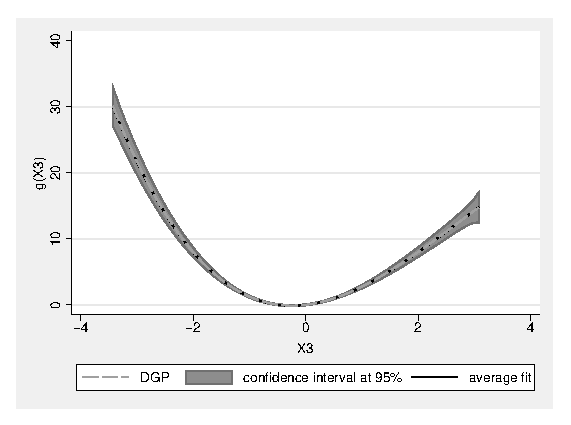
\includegraphics[height=3in]{fig1}
		\caption{Average fit of $g(X_{3})$ across replications}
		\label{fig1}
	\end{centering}
\end{figure}


Next, we consider the case of dynamic panel data (DGP2):

\begin{equation}
Y_{it}=g(U_{it})Y_{it-1}+0.3Y_{it-2}+0.3X_{it}+a_{i}+\varepsilon_{it}
\end{equation}
\begin{equation}
g(U_{it})=sin(\frac{\pi}{3}U_{it})
\end{equation}
\begin{equation}
X_{it}=W_{it}+0.5a_{i}
\end{equation}

We assume $\varepsilon_{it}$ are IID $N(0,1)$ across both $i$ and $t$ and $a_{i}$ are IID $N(0,1)$. $W_{it}$ and $U_{it}$ are drawn from IID $U(0,10)$ and IID $U(-9,9)$, respectively.

We compare the performance of ivxtplfc and ivregress 2sls via the following models:

Model 4: ivxtplfc, considering that $X_{it}$ and $Y_{it-2}$ enter the model linearly, whereas $Y_{it-1}$ is included with a functional coefficient of $U_{it}$.

Model 5: ivregress 2sls, taking first difference to remove fixed effects and regressing $\Delta Y_{it}$ on $\Delta Y_{it-1}$, $\Delta Y_{it-2}$, and $\Delta X_{it}$.

Model 6: ivregress 2sls, taking first difference to remove fixed effects and regressing $\Delta Y_{it}$ on $\Delta Y_{it-1}$, $\Delta Y_{it-2}$, $\Delta X_{it}$ and $\Delta U_{it}$.

It should be noted that $L2.Y_{it}$ (the second lag of $Y_{it}$ ) is used as the instrumental variable in "ivregress 2sls", and the interaction of $L2.Y_{it}$ and the first lag of the basis functions of $U_{it}$ are constructed as the instrumental variables in "ivxtplfc". The simulation codes for DGP 2 are presented as follows:


\begin{stlog}
	
. clear all
{\smallskip}
. set matsize 2000
{\smallskip}
. set obs 50
number of observations (_N) was 0, now 50
{\smallskip}
. set seed 789
{\smallskip}
. gen a=rnormal()
{\smallskip}
. gen id=_n
{\smallskip}
. expand 80
(3,950 observations created)
{\smallskip}
. bys id: gen year=_n
{\smallskip}
. gen x=10*runiform()+0.5*a
{\smallskip}
. gen u=-9+18*runiform()
{\smallskip}
. gen gf=sin(_pi/3*u)
{\smallskip}
. gen y=0
{\smallskip}
. xtset id year
panel variable:  id (strongly balanced)
time variable:  year, 1 to 80
delta:  1 unit
{\smallskip}
. mata: gfmat=J(2000,500,.)
{\smallskip}
. forv j=1/500{\lbr}
2.     
.      preserve
3.     qui replace y=a+0.3*x+0.3*L2.y+L1.y*gf+sqrt(2)*rnormal() if year>2
4.     qui drop if year<41
5.     qui gen L_y=L1.y
6.     qui gen L2_y=L2.y
7.     qui ivxtplfc y L2_y x, zvars(L_y) uvar(u) gen(g) endoz(1) ///
>                                maxnknots(20) ivz(L2_y,uflag(1)) fast brep(500)
8.     qui putmata gfhat=g_1,replace
9.     mata: gfmat[.,`j']=gfhat
10.    matrix B=e(b)
11.    matrix B=B[1,1..2]
12.    matrix B1=(nullmat(B1)\\B)
13.    matrix V=e(Vs)
14.    matrix V=vecdiag(V)
15.    matrix V=V[1,1..2]
16.    matrix V1=(nullmat(V1)\\V)       
17.         
. 
.      qui ivregress 2sls D.y D.L2.y D.x (D.L.y=L2.y), noconstant
18.    matrix B=e(b)
19.    matrix B=B[1,2..3]
20.    matrix B2=(nullmat(B2)\\B)
21.    matrix V=e(V)
22.    matrix V=vecdiag(V)
23.    matrix V=V[1,1..2]
24.    matrix V2=(nullmat(V2)\\V)       
25. 
.      qui ivregress 2sls D.y D.L2.y D.x D.u (D.L.y=L2.y), noconstant
26.    matrix B=e(b)
27.    matrix B=B[1,2..3]
28.    matrix B3=(nullmat(B3)\\B)
29.    matrix V=e(V)
30.    matrix V=vecdiag(V)
31.    matrix V=V[1,1..2]
32.    matrix V3=(nullmat(V3)\\V)               
33.         
.      restore
34. 
. {\rbr}
{\smallskip}
. 
. 
. * Fig 2
. 
. qui drop if year<41
{\smallskip}
. qui getmata (gfs*)=gfmat
{\smallskip}
. egen av_fit = rowmean(gfs*)
{\smallskip}
. egen sd_fit = rowsd(gfs*)
{\smallskip}
. gen  c =  invnormal(1 - (100 - 95) / 200)
{\smallskip}
. gen low = av_fit - c * sd_fit
{\smallskip}
. gen up = av_fit + c * sd_fit
{\smallskip}
. 
.         twoway (rarea low up u, sort(u) color(gs7)) ///
>            (line av_fit u, sort(u) color(black) lpattern(solid)) ///
>            (line gf u, color(gs10) sort lpattern(longdash)), ///
>            legend(label(1 confidence interval at 95\%) label(3 DGP) label(2 average fit) ///
>            cols(3) order(3 1 2)) xtitle("U", height(5)) ytitle("g(U)", height(5)) sch(sj) 
{\smallskip}
. graph2tex , epsfile(fig2) caption(Average fit of g(U)) label(fig2) 
\% exported graph to fig2.eps
\% We can see in Figure \\ref{\lbr}fig:fig2{\rbr} that
\\begin{\lbr}figure{\rbr}[h]
\\begin{\lbr}centering{\rbr}
\\includegraphics[height=3in]{\lbr}fig2{\rbr}
\\caption{\lbr}Average fit of g(U){\rbr}
\\label{\lbr}fig:fig2{\rbr}
\\end{\lbr}centering{\rbr}
\\end{\lbr}figure{\rbr}
{\smallskip}
.         
.         
. * Table 2
. clear
{\smallskip}
. set obs 500
number of observations (_N) was 0, now 500
{\smallskip}
. mat res2=J(3,8,.)
{\smallskip}
. forv k=1/3{\lbr}
2.     qui svmat B`k'
3.     su B`k'1,meanonly
4.     mat res2[`k',1]=r(mean)-0.3
5.     su B`k'2,meanonly
6.     mat res2[`k',2]=r(mean)-0.3
7. 
.      svmat V`k'
8.     qui replace V`k'1=sqrt(V`k'1)
9.     qui gen B`k'1_lb=B`k'1-invnormal(0.975)*V`k'1
10.    qui gen B`k'1_ub=B`k'1+invnormal(0.975)*V`k'1
11.         
.      qui gen CIlen`k'1=B`k'1_ub-B`k'1_lb
12.    qui su CIlen`k'1,d
13.    mat res2[`k',5]=r(p50)  
14.         
.      qui replace V`k'2=sqrt(V`k'2)
15.    qui gen B`k'2_lb=B`k'2-invnormal(0.975)*V`k'2
16.    qui gen B`k'2_ub=B`k'2+invnormal(0.975)*V`k'2
17.         
.      qui gen CIlen`k'2=B`k'2_ub-B`k'2_lb
18.    qui su CIlen`k'2,d
19.    mat res2[`k',6]=r(p50)  
20.         
.      qui gen cov`k'1=(B`k'1_lb<=0.3 \& B`k'1_ub>=0.3) 
21.    su cov`k'1,meanonly
22.    mat res2[`k',7]=r(mean) 
23.         
.      qui gen cov`k'2=(B`k'2_lb<=0.3 \& B`k'2_ub>=0.3) 
24.    su cov`k'2,meanonly
25.    mat res2[`k',8]=r(mean)                         
26.         
.      qui replace B`k'1=(B`k'1-0.3){\caret}2
27.    su B`k'1,meanonly
28.    mat res2[`k',3]=r(mean)
29.    qui replace B`k'2=(B`k'2-0.3){\caret}2
30.    su B`k'2,meanonly
31.    mat res2[`k',4]=r(mean)
32. 
. {\rbr}
{\smallskip}
. outtable using res2, mat(res2)  format(\%9.4f) replace
{\smallskip}	

\end{stlog}


Table \ref{tab2} presents the bias, mean square error (MSE), median width of 95\% confidence interval, and coverage of 95\% confidence interval of the estimated coefficients associated with $Y_{it-2}$ and $X_{it}$. Similar to DGP1, the simulation results show that the fixed-effect sieve 2SLS estimator performs much better than the fixed-effect 2SLS estimator in terms of bias, MSE, width of 95\% confidence interval, and coverage of 95\% confidence interval. Fig. \ref{fig2} displays the average fit of $g(U_{it})$ alongside with the corresponding 95\% band in the simulations. Although $g(U_{it})$ is fluctuated greatly in Model 4, the proposed method estimates it quite well. 


\begin{table*}[htbp]
	
	\scriptsize
	
	\centering
	
	\caption{Simulation results for the parametric parts in DGP 2}
	
	\label{Tab03}
	
	\begin{tabular}{ccccccccc}
		
		\toprule
		
		\multirow{1}{*}{} & \multicolumn{2}{c}{Bias} & \multicolumn{2}{c}{MSE} & \multicolumn{2}{c}{95\% CI width}& \multicolumn{2}{c}{Coverage} \\
		
		\cmidrule(r){2-3} \cmidrule(r){4-5} \cmidrule(r){6-7} \cmidrule(r){8-9}
		
		&  $Y_{it-2}$      &  $X_{it}$   &  $Y_{it-2}$      &  $X_{it}$  & $Y_{it-2}$      &  $X_{it}$ & $Y_{it-2}$      &  $X_{it}$  \\
		
		\midrule
		
		Model 4 &   -0.0009 &   -0.0005 &    0.0002 &    0.0002 &    0.0542 &    0.0527 &    0.9360 &    0.9400 \\ 
		Model 5 &    0.0302 &    0.0357 &    0.0017 &    0.0018 &    0.3623 &    0.2555 &    1.0000 &    1.0000 \\ 
		Model 6 &    0.0266 &    0.0385 &    0.0015 &    0.0020 &    0.3603 &    0.2539 &    1.0000 &    1.0000 \\  
		
		\bottomrule
		
	\end{tabular}
	\label{tab2}	
\end{table*}


\begin{figure}[htbp]
	\begin{centering}
		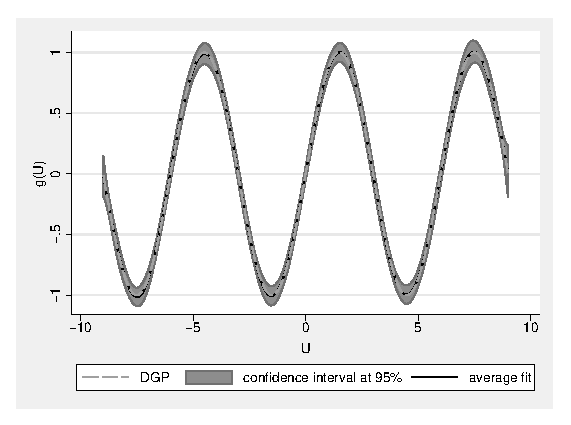
\includegraphics[height=3in]{fig2}
		\caption{Average fit of g(U) across replications}
		\label{fig2}
	\end{centering}
\end{figure}


